\documentclass[11pt,a4paper]{article}

% ------------------------------------------------------------
% Packages
% ------------------------------------------------------------
\usepackage[utf8]{inputenc}
\usepackage[T1]{fontenc}
\usepackage{lmodern}
\usepackage[english]{babel}
\usepackage[a4paper,margin=2.5cm]{geometry}
\usepackage{amsmath,amssymb}
\usepackage{siunitx}
\usepackage{booktabs}
\usepackage{array}
\usepackage{graphicx}
\usepackage{float}
\usepackage{caption}
\usepackage{subcaption}
\usepackage{pgfplots}
\usepackage{pgfplotstable}
\usepackage{xcolor}
\usepackage{enumitem}
\usepackage{hyperref}
\usepackage{microtype}
% \usepackage{siunitx}

% ------------------------------------------------------------
% Custom commands
% ------------------------------------------------------------
\newcommand{\degCel}{\,^\circ\mathrm{C}}
\newcommand{\Frac}[2]{\left(\frac{#1}{#2}\right)}
\setlength{\parindent}{0pt}




\pgfplotsset{compat=1.18}

\sisetup{
    per-mode=symbol,
    exponent-product=\cdot,
    output-decimal-marker={.},
    group-separator={,},
    group-minimum-digits=4
}

\hypersetup{
    colorlinks=true,
    linkcolor=black,
    citecolor=black,
    urlcolor=blue,
    pdftitle={Assignment 5 - Generator Design Tool}
}

% ------------------------------------------------------------
%                       Document information
% ------------------------------------------------------------
\title{
    \textbf{FENT2321}\\[0.3cm]
    Wind Energy and Design of a Wind Turbine\\[0.5cm]
    \Large Assignment 7: Generator Design to match the blades - System design}

\author{Markus Arntzen}
\date{}

\begin{document}

\maketitle
\thispagestyle{empty}

\clearpage
\tableofcontents
\clearpage


% ------------------------------------------------------------
%                       Sections
% ------------------------------------------------------------
\section{Problem 1: Operating point variables}

\subsection{Generator geometry}

\begin{center}
    \renewcommand{\arraystretch}{1.5}
    \setlength{\tabcolsep}{10pt}
    \begin{tabular}{|c|c|}
        \hline
        Poles & 2 \\
        \hline
        Phases & 1 \\
        \hline
        Coils & 4 \\
        \hline
        Length per coil & 26.7m \\
        \hline
        Copper wire diameter & 1.18mm \\
        \hline
        Number of turns per coil & 60 \\
        \hline
    \end{tabular}
\end{center}
    
\subsection{Generator performance}
\subsubsection{Induced voltage at no load}

\begin{center}
    \renewcommand{\arraystretch}{1.5}
    \setlength{\tabcolsep}{10pt}
    \begin{tabular}{|l|c|}
        \hline
        \textbf{RPM} & \textbf{$E_A$ [V]} \\
        \hline
        RPM$_\text{design}$ - 300 & 51.6 \\
        \hline
        RPM$_\text{design}$ & 63.6 \\
        \hline
        RPM$_\text{design}$ + 300 & 75.7 \\
        \hline
    \end{tabular}
\end{center}

\subsubsection{Power curves}
\begin{figure}[h]
    \centering
    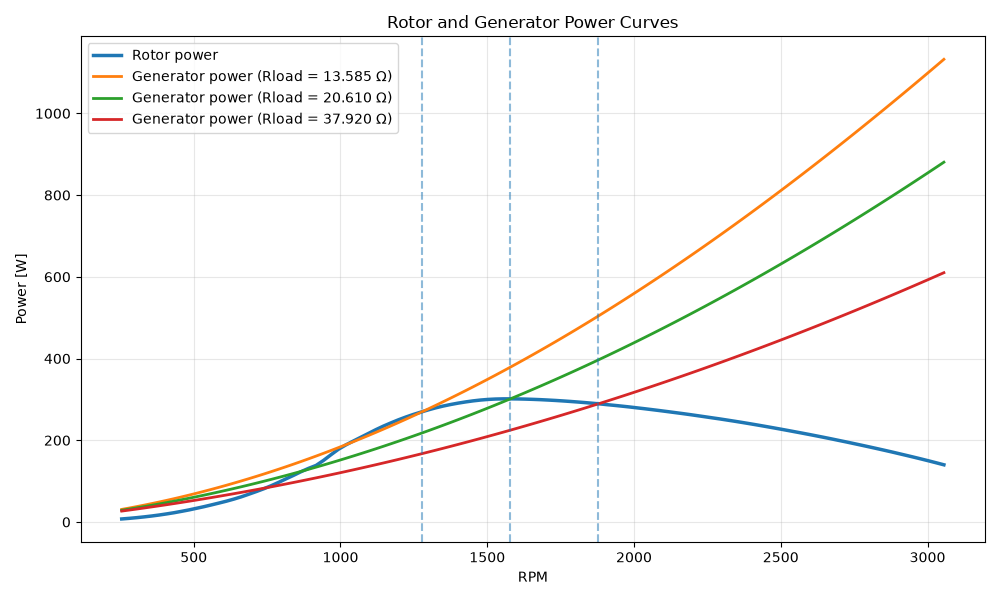
\includegraphics[width=\textwidth]{3.2.2_plot.png}
    \caption{Power curves for different values of $R_{load}$}
    \label{fig:powerPlots}
\end{figure}

\subsubsection{Operating condition parameters}
\begin{center}
    \renewcommand{\arraystretch}{1.5}
    \setlength{\tabcolsep}{5pt}
    \begin{tabular}{|c|c|c|c|c|c|c|c|c|}
        \hline
        RPM
        & $R_L$ [$\Omega$]
        & $P_{el}$ [W]
        & $T_{gen}$ [Nm]
        & $R_A$ [$\Omega$]
        & $X_S$ [$\Omega$]
        & $L_S$ [H]
        & $\eta_{gen}$
        & $\eta_{tot}$ \\
        \hline
        $RPM_{design}-300$
        & 16.465
        & 128.58
        & 1.823
        & 1.877
        & 1.968
        & 0.014694
        & 52.66\%
        & 52.66\% \\
        \hline
        $RPM_{design}$
        & 20.61
        & 163.18
        & 1.823
        & 1.877
        & 2.430
        & 0.014694
        & 54.13\%
        & 54.13\% \\
        \hline
        $RPM_{design}+300$
        & 24.765
        & 197.79
        & 1.823
        & 1.877
        & 2.891
        & 0.014694
        & 55.14\%
        & 55.14\% \\
        \hline
    \end{tabular}
\end{center}

\subsubsection{Discussion}
\begin{itemize}
    \item When $R_L$ is increased, the rotor of the turbine need to output more power.
    Since the torque the wind exerts on the turbine blades remain the same, the
    rotational speed need to increase to increase the power to the generator, thus
    increasing RPM.
    \item If the generator is unable to extract the maximum mechanical power produced
    by the rotor blades, the electrical power output will be limited by the
    generator's capacity. If the rotor produces more mechanical power than the generator
    can absorb, the rotor will accelerate due to the resulting positive torque imbalance.
    This acceleration may shift the tip speed ratio away from its optimal value,
    reducing the aerodynamic efficiency of the rotor. The turbine will therefore be
    unable to convert all the available wind energy into useful electrical power.
    The overall efficiency may decrease due to both the generator limitation and the
    possible deviation from the optimal operating point.
    \item When the wind speed is reduced to half its design value, the wind turbine
    will not necessarily remain at its optimal operating point. For our system,
    the optimal rotor speed would decrease from 1579 rpm to approximately 789.5 rpm
    to maintain the same tip speed ratio. Assuming the rotor maintains its optimal
    power coefficient, the mechanical power available at the design point of 301.47 W
    would decrease to approximately 37.68 W. The corresponding optimal generator torque
    would decrease from 1.823 Nm to approximately 0.456 Nm. However, since the generator
    load resistance is kept constant at 20.61 $\Omega$, the generator torque may not match the
    optimal rotor torque at the reduced wind speed. The actual operating point is
    determined by the intersection of the rotor and generator torque curves.
    Therefore, the turbine will only operate optimally if this intersection occurs
    close to the required rotor speed of 789.5 rpm. Otherwise, the tip speed ratio will
    deviate from its optimal value, reducing the aerodynamic efficiency.
\end{itemize}

\end{document}